\section{Introduction}
\label{sec:intro}

\begin{figure*}[t]
  \centering
  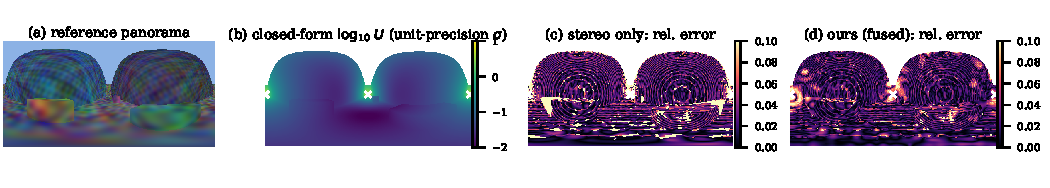
\includegraphics[width=\linewidth]{figures/teaser.pdf}
  \caption{\textbf{Two panoramas see depth only away from the epipoles.} (a) Reference panorama of a
  procedural street; the second panorama was taken 4\,m further down the road. (b) Our closed-form
  triangulation uncertainty at unit matching precision. It blows up at the two epipoles
  (\textcolor{gray}{$\times$}), which look along the street, exactly where the road continues.
  (c) Stereo alone fails in those regions. (d) Weighting stereo by the calibrated uncertainty and
  fusing it with a monocular prior keeps the stereo accuracy where it exists and falls back to the
  prior where it does not.}
  \label{fig:teaser}
\end{figure*}

Street-level panoramas cover most cities many times over. If one or two of them could be turned into
metric 3D geometry close to LiDAR quality, dense city models would become much cheaper to build and to
keep current. Two lines of work come close. Panoramic depth foundation
models~\cite{lin2026dap,da360,pager2026,rey2022360monodepth} predict depth for every direction from a
single image, but even the strongest report relative errors of several percent; at 20\,m that is more
than a metre. Generalizable multi-view methods for
panoramas~\cite{chen2023panogrf,chen2025splatter360,zhang2024pansplat} build spherical cost volumes
from two or more images, but they are trained to synthesize new views, not to produce calibrated metric
geometry.

Two high-resolution panoramas a few metres apart contain far more metric information than either line
of work uses explicitly. That information is spread very unevenly over the sphere, though.
Triangulation error grows with the square of the depth, and it diverges at the \emph{epipoles}, the two
directions along the baseline. A camera on a car or a backpack moves along the street, so the baseline
points down the street, and the region with no parallax is precisely the road ahead and behind
(\cref{fig:teaser}b). A depth estimator that ignores this has two bad options: distrust stereo
everywhere, or trust it in places where it means nothing.

This paper makes that structure explicit and builds the fusion around it. Concretely, we contribute:
\begin{itemize}
  \item A \textbf{closed-form uncertainty} for spherical two-view triangulation, for every ray, that
  also accounts for rotation and translation errors of the relative pose (\cref{sec:sigma}). It agrees
  with Monte Carlo simulation to within 0.5\%.
  \item A \textbf{calibration conditioned on that geometry} (\cref{sec:calibration}). Depth, baseline,
  epipoles, resolution and pose error all stay in the closed form; only the photometric matching
  precision is learned, as a two-parameter monotone map fitted robustly on teacher data.
  \item \textbf{Epipole-aware Bayesian fusion} of a learned panoramic prior with one or more stereo
  partners in log-depth (\cref{sec:fusion}). It corrects the prior's metric scale and rejects
  occlusions and moving objects with a mixture model. It returns metric depth with a per-ray
  uncertainty, and with a single panorama it reduces to the prior.
  \item A \textbf{city-as-teacher} scheme (\cref{sec:teacher}). A dense capture of one city supplies
  triangulation covariances for weighting the supervision, amodal targets behind occluders that only
  other panoramas see, and calibration data. So far we have tested only the last of these uses.
  \item A \textbf{controlled study} against geometry-blind baselines fitted on the same data
  (\cref{sec:experiments}). Without pose error, a well-calibrated match confidence does as well as the
  closed form. With pose error, or with an exposure-robust matching cost, it does not.
\end{itemize}
All experiments use procedural street scenes with exact ground truth. There are \emph{no real-data
experiments} in this draft. \Cref{sec:limitations} describes the KITTI-360~\cite{liao2022kitti360}
protocol with accumulated LiDAR that we consider the most important missing piece.
